\section{Introduction}\label{sec:intro}
An expensive labeling process often leaves a small set of gold-standard outcomes, a larger set of unlabeled observations, and a prediction model that is already fixed. Prediction-powered inference uses the model's scores to improve estimation while correcting their bias with gold-standard labels. In this setting, collecting more labels, replacing the model, and enlarging the unlabeled sample may all be impossible. What precision can still be gained from the same inputs?

We study the population mean. This target has a direct scientific interpretation and makes the source of an improvement transparent: the score can explain variation in the outcome even when its calibration is nonlinear. A scalar correction can miss this information. Conversely, a highly flexible fitted correction can create apparent precision by underestimating its uncertainty. Any useful answer must assess coverage alongside width, and must compare against an efficiently tuned scalar correction rather than only an uncalibrated predictor.

Our answer is conditional. Within a deterministic score-control class, the optimal control is a shrunken conditional mean. A richer fixed basis improves on an unrestricted scalar control only through the additional conditional-mean variation it explains. There is no first-order gain when the conditional mean is affine in the score, and no score-based gain when the score carries no conditional-mean signal. These statements characterize estimator variance within a stated class; they are not a universal lower bound on confidence-interval length.

We evaluate this reasoning through paired repeated-sampling experiments with a frozen score. We distinguish normal-approximation intervals, whose justification is asymptotic, from a bounded-data construction with a finite-sample guarantee. The latter pays for honest nuisance fitting through a training split and for distribution-free concentration through range penalties. Thus an improvement in leading variance does not by itself establish a shorter valid finite-sample interval.

The contribution is a reproducible examination of how much precision remains after scalar tuning, and where it disappears. It combines an explicit variance decomposition, controls for scalar calibration and fitting, empirical-population benchmarks with archived predictions, and a separate finite-sample comparison. The proposed transformations are classical control-variate operations on an existing score; no predictor is retrained and no new labels are acquired.

\section{Related work and positioning}
Prediction-powered inference corrects an imputed estimate with labeled evidence about prediction error, allowing a pretrained black-box predictor to support valid inference \citep{angelopoulos2023ppi}. Its framework includes both normal-approximation procedures and constructions based on finite-sample concentration; calling an interval ``PPI'' alone therefore does not specify its guarantee. Our unit-control baseline is the usual Gaussian mean interval, while the empirical Bernstein comparisons separately address finite-sample validity.

PPI++ introduces power tuning and asymptotically normal estimators for a broad class of targets \citep{angelopoulos2024ppipp}. For means, power tuning learns a scalar control coefficient. Its discussion also explicitly connects prediction-powered estimators to augmented inverse-propensity estimation and the conditional-mean nuisance function, including the $1/(1+n/N)$ shrinkage factor. We use this established connection rather than claim a new semiparametric principle. Our narrower question concerns what a fixed low-dimensional nonlinear transformation of an already frozen scalar score can add beyond scalar tuning, after paying for fitting and checking coverage.

Cross-prediction-powered inference uses labeled folds to train prediction models while evaluating their corrections on held-out data \citep{zrnic2024cross}. Here the original prediction model remains fixed: cross-fitting applies only to the small inferential regression on its scalar output. We consequently make no claim of introducing cross-fitting or of evaluating the full cross-prediction method with newly trained predictors. The empirical Bernstein construction uses the known-range inequality of \citet{maurer2009empirical}; its guarantee comes from independent training and concentration, rather than from a Gaussian approximation. The study's contribution is the controlled comparison, explicit conditions, and reproducible evidence at this fixed-input scope.

Stratified PPI exploits conditional heterogeneity through a prespecified partition, fixed within-stratum sample counts, and masses treated as known \citep{fisch2024stratified}. Retrospective iid draws instead have random stratum counts and finite-$N$ mass uncertainty; importing its allocation benefit or treating estimated masses as fixed would change this comparison. We do not evaluate an iid poststratified/bin-indicator control, and claim no superiority over it or all nonlinear controls. Active statistical inference improves precision by choosing which labels to acquire \citep{zrnic2024active}; label identities are already fixed here, so that acquisition advantage is outside our setting.


\section{Problem and inferential scope}\label{sec:problem}
Let $S=f(X)$ be a scalar score from a frozen predictor. We observe $L=\{(Y_i,S_i)\}_{i=1}^n$ and $U=\{\widetilde S_j\}_{j=1}^N$, drawn independently and identically within and between samples from a common population. The target is $\mu=\mathbb E[Y]$. Each procedure receives exactly the same $L,U$ and frozen $f$ in each repetition. A procedure may fit an inferential transformation of $S$ using the available labels, but may not acquire labels, replace $f$, or augment $U$.

``Fixed'' describes the comparison of procedures on a draw. Frequentist coverage concerns repetitions of the sampling experiment; it does not assign a sampling probability to one fully conditioned-on data set. We do not study confidence conditional on every observed label and score, adaptive label acquisition, distribution shift, or uncertainty in a newly trained prediction model.

The empirical-data experiments use each archived record list as a discrete empirical population. Labeled and unlabeled indices are sampled independently with replacement, and the mean of all archived labels is the benchmark truth. This gives a known target and the same sampling model as the synthetic experiments. It does not establish inference for a broader scientific population. Repeated indices are permitted by that sampling law. The evaluation harness uses all archived labels to define truth; estimators receive only their selected labeled outcomes.

\section{How much improvement is available?}\label{sec:method}
\subsection{A score-control variance identity}
For deterministic $h$, consider
\begin{equation}
 \widehat\mu_h=\frac1n\sum_{i=1}^n\{Y_i-h(S_i)\}
 +\frac1N\sum_{j=1}^N h(\widetilde S_j).
 \label{eq:estimator}
\end{equation}
Under common-population sampling and finite second moments, this estimator is unbiased and has variance
\begin{equation}
 V(h)=\frac{\operatorname{Var}(Y-h(S))}{n}
       +\frac{\operatorname{Var}(h(S))}{N}.
 \label{eq:variance}
\end{equation}
Let $r=n/N$ and $m(S)=\mathbb E[Y\mid S]$. Constants in $h$ cancel in~\eqref{eq:estimator}. Completing the square yields
\begin{align}
 V(h)&=\frac{\operatorname{Var}(Y)}n
 -\frac{\operatorname{Var}(m(S))}{n(1+r)}\nonumber\\
 &\quad+\frac{1+r}{n}\operatorname{Var}\left(h(S)-\frac{m(S)}{1+r}\right).
 \label{eq:identity}
\end{align}
Thus $h^*(S)=m(S)/(1+r)$, up to a constant, minimizes variance in this class, giving
\begin{equation}
 V^*=\frac{\mathbb E[\operatorname{Var}(Y\mid S)]}{n}
        +\frac{\operatorname{Var}(m(S))}{n+N}.
 \label{eq:optimum}
\end{equation}
Even perfect prediction leaves finite unlabeled-sample uncertainty. Transforming one score repeatedly does not create new independent observations.

For scalar $h(S)=aS$, the optimum is
\begin{equation}
 a^*=\frac{\operatorname{Cov}(Y,S)}{(1+r)\operatorname{Var}(S)}
 \label{eq:scalar}
\end{equation}
when $\operatorname{Var}(S)>0$. If the score is constant, it cannot help. Let $\Pi_1m$ and $\Pi_pm$ be the centered $L^2$ projections of $m$ onto a scalar score and a nested, fixed $p$-dimensional basis. The decrease in optimal variance is
\begin{equation}
 V_1^*-V_p^*=\frac{\operatorname{Var}(\Pi_pm)-\operatorname{Var}(\Pi_1m)}{n(1+r)}.
 \label{eq:projection}
\end{equation}
An affine conditional mean leaves no additional projection signal. A nonlinear conditional mean can yield a strict gain, but only if the chosen basis represents its additional variation. These oracle comparisons do not pay for estimating coefficients and do not imply that fitted intervals improve for every $n$.

\subsection{Fitted controls and normal-approximation intervals}
Our richer control uses three prespecified Legendre coordinates on $[0,1]$, excluding the intercept. Two fixed equal folds alternate between fitting centered least squares on one half of the labeled observations and evaluating residuals on the other half. Each fitted coefficient vector is multiplied by $1/(1+n/N)$. The estimator averages the held-out corrections and uses the corresponding average control on all $N$ unlabeled scores.

The standard error combines the empirical variance of out-of-fold residuals divided by $n$ and the variance of the averaged unlabeled control divided by $N$. We use two-sided Gaussian intervals. With fixed basis dimension, nonsingular population basis covariance, consistent coefficients, finite second moments, positive limiting oracle variance, and $n,N\to\infty$ at positive finite ratio, the product of coefficient error with the held-out labeled/unlabeled basis-mean difference is $o_p(n^{-1/2})$: coefficient consistency gives $o_p(1)$ error, while the mean difference is $O_p(n^{-1/2})$. The interval then has the oracle fixed-basis normal limit. Cross-fitting protects held-out residual evaluation from direct training reuse; it does not give exact finite-sample coverage.

We compare label-only normal intervals, unit-control PPI, the pinned PPI++ scalar implementation, an unrestricted scalar, and cross-fitted linear and cubic controls. The unrestricted scalar separates nonlinear gains from restrictions imposed by clipping the scalar tuning parameter to $[0,1]$. Cross-fitted linear controls help separate nonlinear representation from the cost of splitting and fitting. A cubic fitted and evaluated on the same labels and prespecified degree-12 controls diagnose overfitting. No basis dimension is selected from the reported coverage or width results.

\subsection{A finite-sample bounded-data construction}
Suppose $Y,S\in[0,1]$. For $k\ge2$ independent identically distributed observations $Z$ in a known interval of length $R$, with unbiased sample variance $v_Z$, define
\begin{equation}
 b(Z,R,\delta)=\sqrt{\frac{2v_Z\log(4/\delta)}k}
             +\frac{7R\log(4/\delta)}{3(k-1)}.
 \label{eq:bernstein}
\end{equation}
Applying the empirical Bernstein inequality to $Z$ and its reflection yields a two-sided interval with failure probability at most $\delta$. The additive range term matters even if observed residual variance is small.

Reserve $\max(10,\lfloor n/4\rfloor)$ labeled observations for fitting; let $m\ge2$ be the remaining count and require $N\ge2$. Conditional on training, choose a fixed control $h\in[0,c]$. Residuals lie in $[-c,1]$, with known length $1+c$. A valid radius for~\eqref{eq:estimator}, now using $m$ evaluation labels, is
\begin{equation}
 b(Y-h(S),1+c,\alpha/2)
 +b(h(\widetilde S),c,\alpha/2).
 \label{eq:finite}
\end{equation}
A conditional union bound and then averaging over training give coverage at least $1-\alpha$. Intersecting the interval with $[0,1]$ preserves coverage. No correctness of the fitted regression is needed.

We use a clipped scalar and a clipped cubic regression trained only on the reserved labels, with shrinkage $1/(1+m/N)$. All training labels count toward the original $n$-label budget. The label-only empirical Bernstein baseline uses all $n$ labels. A unit-control baseline also uses all $n$ labels because it requires no fitting; a common-split version exposes the split's cost. Binary outcomes additionally permit exact label-only Clopper--Pearson intervals. These comparisons address finite-sample validity directly; they should not be pooled with asymptotically justified Wald intervals as if all guarantees were interchangeable.

\section{Experimental design}\label{sec:design}
All methods are paired on identical draws. The main grid uses $n\in\{100,500,2000\}$, $N=10n$, and 5,000 independent repetitions per setting. Seven synthetic regimes cover linear and nonlinear calibration, no signal, heavy-tailed noise, nonlinear Bernoulli responses and rare events. Three archived binary-outcome datasets supply frozen scores for galaxy morphology, forest loss and protein disorder. A separately specified high-signal bounded quadratic experiment uses $n\in\{2000,10000\}$ and 3,000 repetitions to study whether finite-sample range penalties can be overcome. Generating mechanisms, seeds and sampling details are in Appendix~\ref{app:reproduction} and the supplied code. The complete study contains 165,000 draw sets over 35 scenario/sample-size cells; all 1,935,000 method records are retained.

Coverage is the fraction of intervals containing the known mean; its uncertainty is a 95\% Wilson Monte Carlo interval. Average widths have Monte Carlo standard errors. A relative width is the ratio of paired mean widths, not the average of within-repetition ratios. Its standard error uses the paired delta method. A narrow interval is not judged preferable when it undercovers. Coverage near 95\% in a finite simulation is evidence about the tested setting, not a proof of validity. Exploratory one-sided exact-binomial undercoverage tests use Holm adjustment across all cells separately for each method. The family is the completed study grid, not a distribution-uniform test.

\section{Results}\label{sec:results}
Figures~\ref{fig:main} and~\ref{fig:finite} pair coverage with width; Appendix~\ref{app:displays} reports sample-size trends and diagnostics, and Appendix~\ref{app:complete} retains every completed method/setting cell.
\begin{figure}[t]
\centering
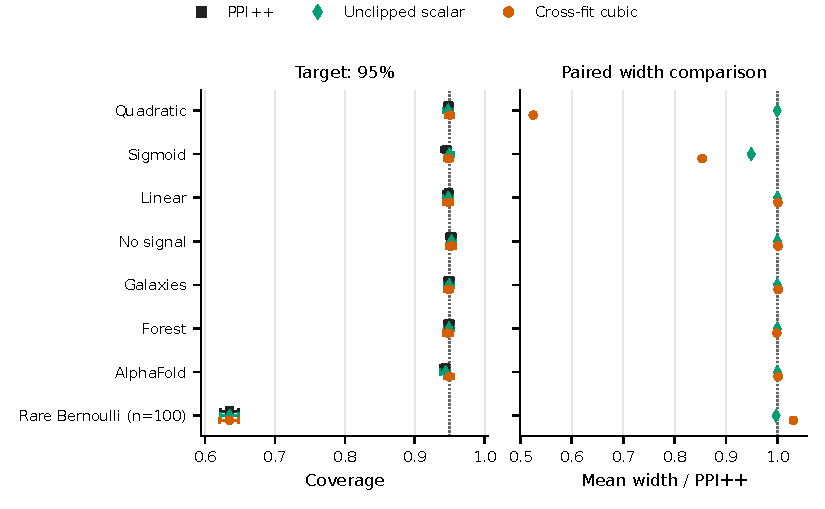
\includegraphics[width=\linewidth]{figures/main_comparison.pdf}
\caption{Nonlinear gains, no-gain controls, archive results and a small-sample failure. Scalar PPI++ (\texttt{ppi-python 0.2.3}), unrestricted scalar and cross-fitted cubic use identical inputs. All rows have $n=2000,N=20000$, except rare Bernoulli ($n=100,N=1000$); $R=5000$ repetitions per row. Left: coverage with 95\% Wilson Monte Carlo intervals. Right: ratios of paired mean widths to PPI++, with 95\% delta-method Monte Carlo intervals. Rare-event short intervals fail. The archive rows use independent with-replacement draws and target empirical archive means, with no broader population claim. These Wald intervals have asymptotic justification, not finite-sample guarantees.}
\label{fig:main}
\end{figure}
\paragraph{Nonlinear signal can leave substantial precision after scalar tuning.}
For quadratic Gaussian regression at $n=2000$, $N=20000$, the cubic/PPI++ ratio of mean widths is \QuadRatio{} (paired 95\% Monte Carlo interval \QuadRatioCI{}), a \QuadReduction{} reduction. Cubic coverage is \QuadCoverage{} (Wilson interval \QuadCoverageCI{}); PPI++ coverage is \QuadBaseCoverage{} (\QuadBaseCoverageCI{}). Both are compatible with the nominal target, while neither has an exact finite-sample guarantee. Against the unrestricted scalar, the ratio is \QuadUnclippedRatio{} (\QuadUnclippedRatioCI{}), so clipping is not the explanation. The predicted leading-order oracle ratio is $0.524$, closely matching the fitted result. Linear and no-signal cases instead give cubic/PPI++ ratios \LinearRatio{} and \NoSignalRatio{}, respectively, consistent with a small fitting cost and no first-order nonlinear benefit. These controls matter as much as the designed positive case.

\paragraph{Finite unlabeled information limits the gain.}
A documented follow-up after the initial real/bounded results repeats linear, quadratic and no-signal regimes with $n=N=2000$, using 3,000 repetitions. The quadratic ratio becomes \QuadEqualRatio{} (\QuadEqualRatioCI{}), close to the analytical prediction $0.775$, with cubic coverage \QuadEqualCoverage{} (\QuadEqualCoverageCI{}). The reduction from the $N=10n$ gain agrees with the second term in~\eqref{eq:optimum}; it does not establish performance at untested sample ratios.

\paragraph{Archived-data results show no practical nonlinear gain.}
At $n=2000$, cubic/PPI++ ratios are \GalaxyRatio{} (\GalaxyRatioCI{}) for galaxies, \ForestRatio{} (\ForestRatioCI{}) for forest, and \AlphaFoldRatio{} (\AlphaFoldRatioCI{}) for AlphaFold. Cubic coverage is \GalaxyCoverage{}, \ForestCoverage{}, and \AlphaFoldCoverage{}, respectively; their Wilson intervals include $.95$. The small forest reduction is approximately one tenth of one percent; the other two widen. At $n=500$ all three widen. These results concern the empirical distributions of archived labels and frozen predictions, with independent with-replacement draws. They support no claim of broader natural-population coverage or useful real-data shortening.

\paragraph{A narrow normal interval can fail badly.}
For rare Bernoulli outcomes with prevalence $.01$ and $n=100$, cubic coverage is \RareCoverage{} (\RareCoverageCI{}), label-only Wald coverage is \RareLabelCoverage{} (\RareLabelCoverageCI{}), and exact Clopper--Pearson coverage is \RareExactCoverage{} (\RareExactCoverageCI{}). The apparent Wald precision is inadmissible for the task's validity requirement. Zero-width intervals when all selected labels are zero remain in the summaries. The exploratory Holm-adjusted undercoverage diagnostic flags cubic intervals for galaxies and AlphaFold at $n=100$, and rare Bernoulli at $n=100,500$. Failure to reject in other cells is not a coverage certificate.

Cross-fitting also leaves nuisance-fit instability: at $n=100$, forest cubic widths have median $.131636$ and maximum $35.827096$, while AlphaFold has median $.101198$ and maximum $8.748830$. These large intervals are retained in means and uncertainty. Degree-12 and same-label plug-in diagnostics further expose fitting costs; they are not presented as automatically valid competitors.

\begin{figure}[t]
\centering
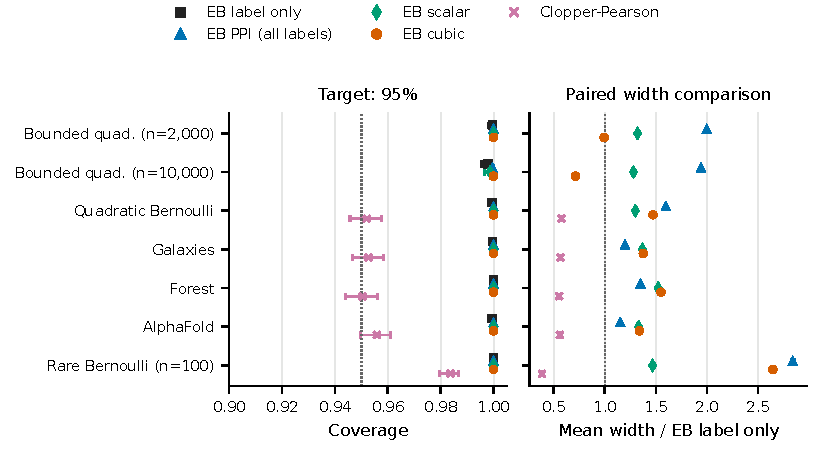
\includegraphics[width=\linewidth]{figures/finite_comparison.pdf}
\caption{Finite-sample guarantees can coexist with gains or substantial conservatism. EB methods have bounded-data guarantees under independent iid sampling; trained controls reserve labels from the original budget, while label/fixed-PPI baselines use all $n$. CP is exact binary label-only and is absent for nonbinary bounded rows. All rows have $n=2000,N=20000$, except labeled $n=10000$ bounded ($N=100000$) and $n=100$ rare-event ($N=1000$) rows. Bounded rows use $R=3000$; binary rows use $R=5000$. Left: empirical coverage with 95\% Wilson Monte Carlo intervals. Right: paired mean-width ratios to EB label-only with 95\% delta-method Monte Carlo intervals. The designed bounded case gains; archived empirical populations do not. These Monte Carlo intervals are distinct from target-mean intervals and theorem guarantees. This compares the stated EB/CP family.}
\label{fig:finite}
\end{figure}
\paragraph{Finite-sample guaranteed shortening is possible, but conservative.}
In the high-signal bounded-quadratic supplement, $n=10000$, $N=100000$, cubic EB/label-only EB mean-width ratio is \BoundedRatio{} (\BoundedRatioCI{}), a \BoundedReduction{} reduction. Against all-label unit-PPI EB it is \BoundedUnitRatio{} (\BoundedUnitRatioCI{}), and against trained scalar EB it is \BoundedScalarRatio{} (\BoundedScalarRatioCI{}). Cubic EB mean width is \BoundedWidth{} (Monte Carlo SE \BoundedWidthSE{}), and all 3,000 intervals cover (Wilson interval \BoundedCoverageCI{}). The $\ge95\%$ guarantee follows from boundedness and independent training, not this hit count. At $n=2000$, the ratio to label-only EB is \BoundedSmallRatio{} (\BoundedSmallRatioCI{}): range penalties nearly erase the gain.

On all three empirical populations, cubic EB is wider than label-only EB, all-label unit-PPI EB, scalar EB, and exact Clopper--Pearson. In the nonlinear Bernoulli case it can beat unit-PPI EB while losing to label-only EB and Clopper--Pearson. Thus the finite-sample success is limited to a designed high-signal setting and the measured EB comparator family. These conservative intervals also remain substantially wider than their Wald counterparts; comparing across guarantee classes cannot remove that cost.


\section{Discussion and limitations}\label{sec:limitations}
The value of a frozen predictor depends on the information in its score, rather than its raw prediction accuracy alone. A scalar correction can leave nonlinear conditional-mean information unused. However, the extra fit consumes statistical precision, and at small label counts it can erase an oracle gain or invalidate a normal approximation. A no-signal score provides no mean-estimation advantage in the deterministic control class. An affine conditional mean leaves scalar tuning first-order optimal in that class.

Finite-sample validity imposes a different price. Known-range concentration and independent training provide a robust guarantee for bounded outcomes, but conservative range terms and label splitting can dominate variance savings. A finite-sample positive result in a designed high-signal regime does not establish improvement for all bounded populations, nor does empirical coverage validate an unproved Gaussian interval.

Our analysis is restricted to means and scalar frozen scores. It does not establish global optimality over all estimators or confidence sets, inference under distribution shift, conditional-on-the-observed-sample validity, robustness to adaptive basis selection, or generalization beyond the archived empirical populations. Synthetic mechanisms expose possibilities and failures under a known law; they cannot determine their prevalence in scientific practice. The practical lesson is to examine additional explainable variation, coefficient-estimation cost and coverage together before claiming precision gains.


\paragraph{Broader impacts.} Using a frozen score more effectively can reduce the precision cost of expensive labeling. The main risk is overconfident scientific or policy inference when a short interval undercovers, or when an archived-data result is generalized beyond its sampling population. Reporting failures, separating guarantee classes and retaining reproducible coverage diagnostics are essential safeguards against that misuse; this work does not validate deployment in any particular scientific or policy setting.
